\newpage
\section{Grafi}
\subsection{Grafo orientato}
\begin{definition}[Grafo orientato]
Un grafo orientato è una relazione $E: V \leftrightarrow V$ su un insieme finito $V$. In un grafo $V$ è l'insieme di nodi o vertici, $E$ è l'insieme di archi o lati. Chiamiamo $G$ (o $G^1$, $G_1$, $G_2$) e scriviamo $G = (V,E)$
\end{definition}
 

\begin{example}\label{esempio-grafo-1}
    Qui di seguito un esempio di un grafo:
\end{example}
 
\hspace{-15pt}Dati i due insiemi $V$ e $E$:\\\\
$V = \{0,1,2,3,4,5\}$ \\
$E = \{(0,0), (0,1), (0,5), (1,3), (1,5), (2,1), (3,4), (3,5), (5,3), (5,4)\}$\\ \\
\begin{wrapfigure}[4]{r}{5cm}
    \vspace{-100pt}
    \centering
    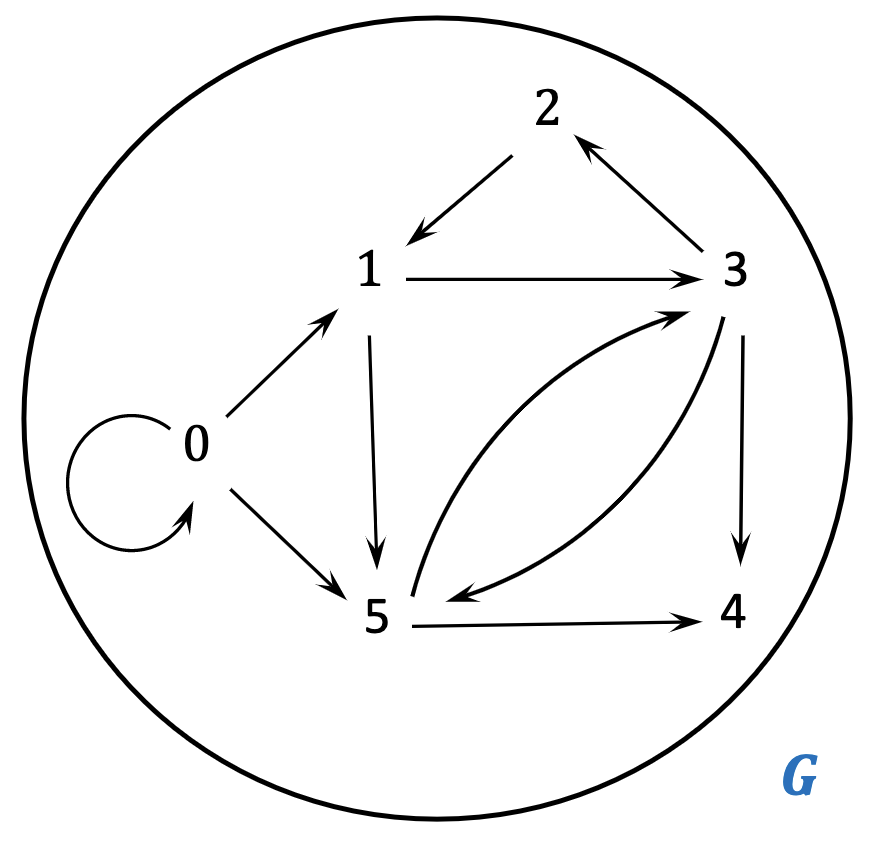
\includegraphics[width=3.7cm]{images/esempio-grafo.png}
    \vspace{-5pt}
    \caption{Grafo G}
    \label{fig:esempio-grafo}
\end{wrapfigure}
Quello rappresentato nell'immagine \ref{fig:esempio-grafo} è un grafo orientato.\\
In questo esempio $n = 6$ e $m = 10$ mentre l'arco $(0,0)$ è un cappio.

\subsubsection{Notazione sui grafi orientati}
Alcune punti di notazione e definizioni sui grafi (Esempi riferiti a immagine \ref{fig:esempio-grafo}):
\begin{itemize}
    \item \textbf{Cardinalità nodi}: $n = \lvert V \rvert $. \hspace{.5cm} \textbf{Cardinalità archi}: $m = \lvert E \rvert$. \hspace{.5cm} $V = \lvert V\rvert = \{0,1,\ldots, \lvert V\rvert-1\}$
    \item \textbf{Cappio}: Un arco $(1,1)$ quindi che parte e ritorna allo stesso nodo lo chiamiamo \textbf{cappio}.
    \item \textbf{Nodi adiacenti}: Nodi $x,y \in V$ sono detti \textbf{adiacenti} se $(x,y) \in E \lor (y,x) \in E$
    \item \textbf{Vicinato in uscita} di $x \in V$: \hspace{.7cm} $N^+(x) = \{y \mid (x,y) \in E\}$.
    \begin{example}
        $N^+(1) = \{3,5\}$.
    \end{example}
    \item \textbf{Vicinato in ingresso} di $x \in V$: \hspace{.7cm} $N^+(x) = \{y \: | \: (y,x) \in E\}$.
    \begin{example}
        $N^-(1) = \{0,2\}$.
    \end{example}
    \item \textbf{Grado di uscita}: dato un nodo $x \in V$: \hspace{.7cm} $d^+_x = |N^+(x)|$.
    \begin{example}
        $d^+_0 = 3$, $d^+_4 = 0$.
    \end{example}
    \item \textbf{Grado di ingresso}: dato un nodo $x \in V$: \hspace{.7cm} $d^-_x = |N^-(x)|$.
    \begin{example}
        $d^+_5 = 3$.
    \end{example}
\end{itemize}

\begin{definition}[Pozzo, sorgente, isolato]
    Definiamo un nodo si dice \textbf{sorgente} se non ha archi entrati, si dice \textbf{pozzo} se non ha archi uscenti e si definisce \textbf{isolato} se non ha ne archi uscenti ne entrati.
\end{definition}

\subsubsection{Grafi orientati come relazioni e proprietà TUSI}
Vediamo ora le quattro proprietà viste per le relazioni (Totale, univalente, surgettiva, iniettiva) come si applicano ai grafi. Dato un grafo orientato $E: V \leftrightarrow V$ possiamo dire che:
\begin{enumerate}
    \item $E: V \leftrightarrow V$ è \textbf{totale} $\Longleftrightarrow$ per ogni nodo $x \in V$ vale $d^+_x \geq 1$.
    \item $E: V \leftrightarrow V$ è \textbf{univalente} $\Longleftrightarrow$ per ogni nodo $x \in V$ vale $d^+_x \leq 1$.
    \item $E: V \leftrightarrow V$ è \textbf{iniettiva} $\Longleftrightarrow$ per ogni nodo $x \in V$ vale $d^-_x \geq 1$.
    \item $E: V \leftrightarrow V$ è \textbf{surgettiva} $\Longleftrightarrow$ per ogni nodo $x \in V$ vale $d^-_x \leq 1$.
\end{enumerate}

\subsubsection{Hand-shaking lemma}
\begin{proposition}[Hand-shaking lemma]
Per ogni grafo orientato $G = (V,E)$, vale che:
\begin{equation}\label{hand-shaking-lemma}
    \sum\limits_{x \in V}d^-_x \: \: \: = \: \: \: \sum\limits_{x \in V}d^+_x \: \: \: = \: \: \: |E|
\end{equation}
\end{proposition}
Questo lemma può essere dimostrando intuitivamente. Se infatti prendiamo un qualsiasi arco fra esso per forza avrà un nodo di partenza ed uno di fine, quindi si dovrà per forza fare un "+1" sia alla somma degli archi entrati, alla somma degli uscenti, che alla somma di tutti gli archi, se questa cosa la estendiamo a tutti gli archi di un grafo possiamo scrivere allora scrivere che $\sum\limits_{x \in V}d^-_x = \sum\limits_{x \in V}d^+_x = |E|$.
\begin{demostration}
Andiamo a dimostrare questa proprietà in modo più formale per induzione:
\begin{enumerate}
    \item \underline{Caso base:} Se $\lvert E\rvert = 0$ non ci sono archi quindi il grado di uscita di ogni nodo sarà per forza 0, e quindi anche la somma di tutti i gradi in uscita sarà 0.
    \begin{center}
        $\sum\limits_{x \in V}d^+_x = 0 = \lvert E\rvert $
    \end{center}
    \item \underline{Passo induttivo:} Supponiamo che la proprietà valga per tutti i grafi con $m$ archi, noi dobbiamo dimostrare il caso $m+1$. \\
    Prendiamo ora un grafo $G = (V,E)$ con $\lvert E\rvert = m+1$, essendo che $\lvert E \rvert > 0$ esiste per forza almeno un arco. Ora rimuoviamo da questo grafo un arco casuale $(i,j) \in E$ tale che si vada a creare un nuovo grafo $G' = (V, E')$ con $E' = E \setminus \{(i,j)\}$, inoltre possiamo anche vedere che in questo nuovo grafo $\lvert E'\rvert = \lvert E\rvert - 1$ che è uguale a $\lvert E'\rvert = m$.\\\\
    Avendo supposto che la proprietà per ogni $m$ sia vera abbiamo che $\sum_{x\in V}d'^+_x = \lvert E'\rvert$. 
    \\Ora noi sappiamo che se escludiamo per esempio $i$ dai nodi abbiamo che $d^+_x = d'^+_x$ per ogni $x \in V \setminus \{ i \}$, mentre $d^+_i = d'^+_i + 1$ perché in $d^+_i$ consideriamo un uscente in più che in $d'^+_i$ non abbiamo e quindi dobbiamo aggiungere. Risulta che quindi se sommiamo i gradi in uscita di $G$ in risultato sarà uguale alla somma dei gradi uscenti di $G'$ + il numero di archi di differenza (in questo caso 1) quindi:
    \begin{center}
        $\sum\limits_{x \in V}d^+_x = \sum\limits_{x \in V}d'^+_x + 1 = \lvert E'\rvert + 1 = \lvert E\rvert $
    \end{center}
    E così dimostrata questa proposizioni tramite induzione. $\blacksquare$
\end{enumerate}
\end{demostration}

\subsection{Rappresentazione grafi}
\begin{figure}[h!]
    \centering
    \begin{subfigure}{.3\textwidth}
        \centering
        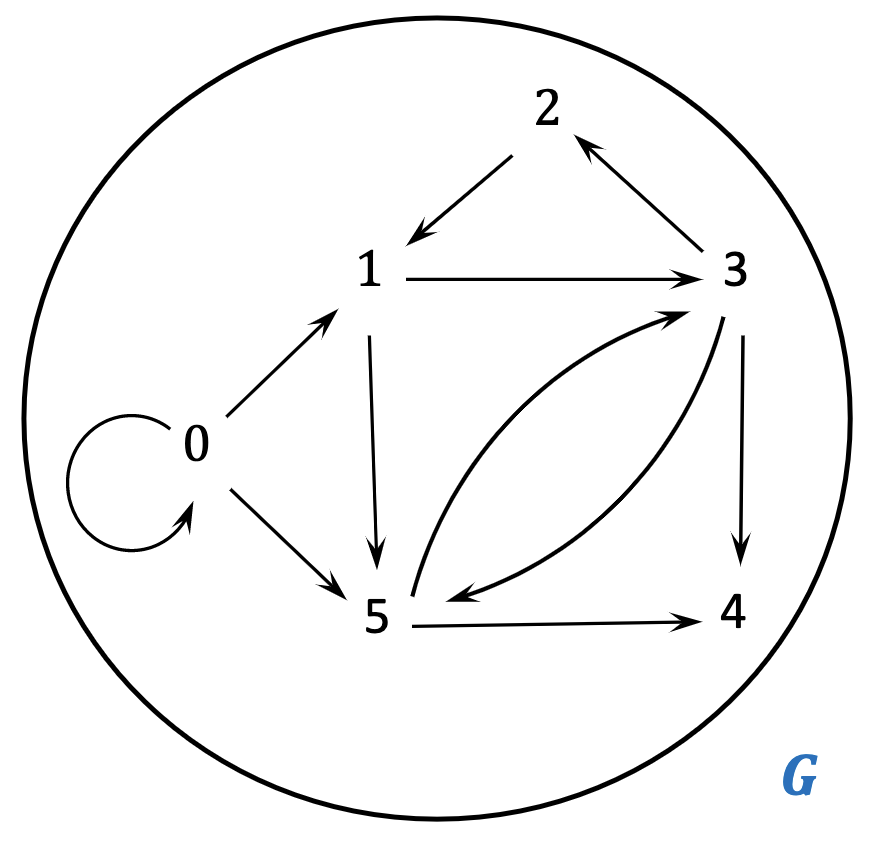
\includegraphics[width=3.3cm]{images/esempio-grafo.png}
        \caption{}
    \end{subfigure}
    \hfill
    \begin{subfigure}{.3\textwidth}
        \centering
        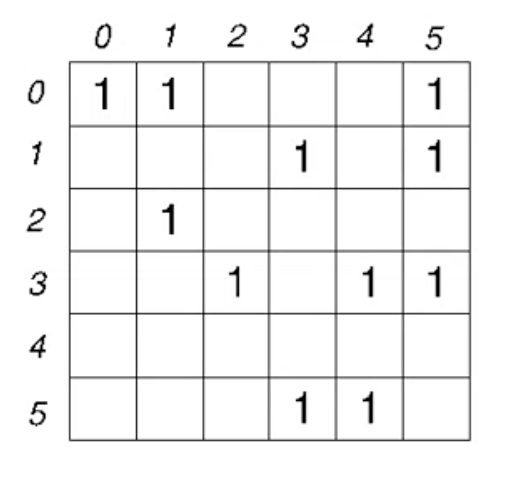
\includegraphics[width=3.3cm]{images/matrice-adiacenza.png}
        \caption{}
    \end{subfigure}
    \hfill
    \begin{subfigure}{.3\textwidth}
        \centering
        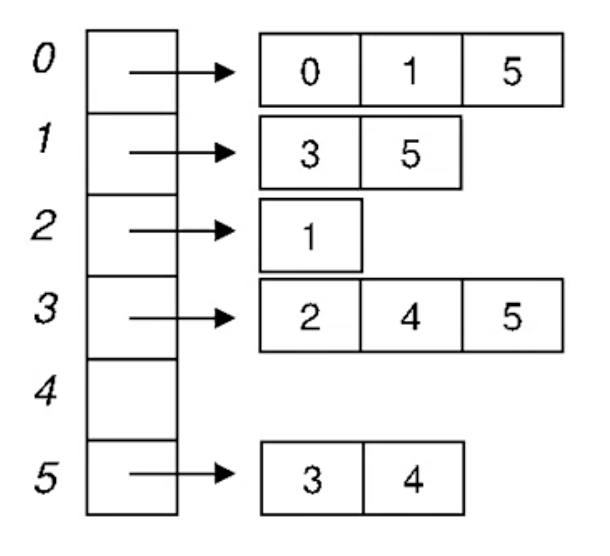
\includegraphics[width=3.3cm]{images/liste-adiacenza.png}
        \caption{}
    \end{subfigure}
    \vspace{-5pt}
    \caption{In (a) il grafo, in (b) la matrice di adiacenza ed in (c) la lista di adiacenza}
\end{figure}
\subsubsection{Matrici di adiacenza}
Una delle tecniche di rappresentazione di un grafo è tramite una matrice di adiacenza.
\begin{definition}[Matrice di adiacenza]
    La matrice di adiacenza di $G$ è una matrice quadrata $A$ con $n$ righe e $n$ colonne, numerate da $0$ a $n-1$, dove l'elemento di $A_ij$ (in riga $i$ e colonna $j$) assume un valore in $0$ se $(i,j) \notin E$ e $1$ se $(i,j) \in E$.
\end{definition}
Questo tipo di rappresentazione è molto utile per sfruttare tecniche di algebra lineare, ma non conviene in termine di spazio occupato se ci sono pochi archi da rappresentare.\\
Alcune proprietà dei grafi viste tramite le matrici di adiacenza:
\begin{itemize}
    \item Dato $x \in V$, $N^+(x)$ si ottiene guardando tutti gli $1$ nella riga $x$.
    \item Dato $x \in V$, $N^-(x)$ si ottiene guardando tutti gli $1$ nella colonna $x$.
    \item Per ottenere $|E|$ si sommano tutti gli $1$ nella matrice.
    \item $d^+_x$ si ottiene sommando gli $1$ di una riga.
    \item $d^-_x$ si ottiene sommando gli $1$ di una colonna.
\end{itemize}

\subsubsection{Liste di adiacenza}
Un metodo alternativo alle matrici di adiacenza sono le liste di adiacenza.
\begin{definition}[Liste di adiacenza]
    La rappresentazione con liste di adiacenza di un grafo orientato $G = (V,E)$ è costituita da un array di $A$ di $n = |V|$ insiemi in cui l'elemento i-esimo è il vicinato in uscita del nodo $i \in V$, cioè $A[i] = N^+(i)$.
\end{definition}
Questo tipo di rappresentazione occupa meno memoria delle matrici di adiacenza se $|E|$ è molto minore di $|V|^2$. Questo perché se prendiamo per esempio una $|E| = 10^{11}$ ed una $|V| = 10^9$ la rappresentazioni di una matrice occuperà $|V|^2$ spazi che sono uguali a $10^{18}$ mentre le liste occuperanno spazi uguali a $|V| + |E|$ che in questo caso sarebbero $10^9 + 10^{11}$ che è minore di della rappresentazione della matrice.\\
Alcune proprietà dei grafi viste tramite le matrici di adiacenza:
\begin{itemize}
    \item Dato $x \in V$, $N^+(x)$ si ottiene leggendo semplicemente la lista di adiacenza ad $x$.
    \item Dato $x \in V$, $N^-(x)$ si ottiene leggendo tutte le di di adiacenza e cercando occorrenze di $x$.
\end{itemize}

\subsection{Grafi orientati etichettati e pesati}
\begin{definition}[Grafo etichettato, grafo pesato]
    Un grafo orientato, etichettato o pesato è una tripla $G = (V,E,L)$ dove $L$ è una funzione $L: (V \cup E) \to D$ che associa ad ogni nodo e arco una etichetta presa da un certo dominio $D$ di valori. Nel caso che $D$ sia un valore numeri il grado si chiama anche pesato.
\end{definition}
La rappresentazioni di etichette su grafi orientati è simile a quella per grafi normali, quindi si possono usare le tecniche di matrici di adiacenza e di liste di adiacenza andando però nel primo caso ad aggiungere l'etichetta al posto del numero 1, mentre nelle liste di adiacenza gli elementi dell'array conterranno una coppia di valori: il nodo a cui è collegato e il valore dell'etichetta.
\begin{figure}[h!]
    \centering
    \begin{subfigure}{.3\textwidth}
        \centering
        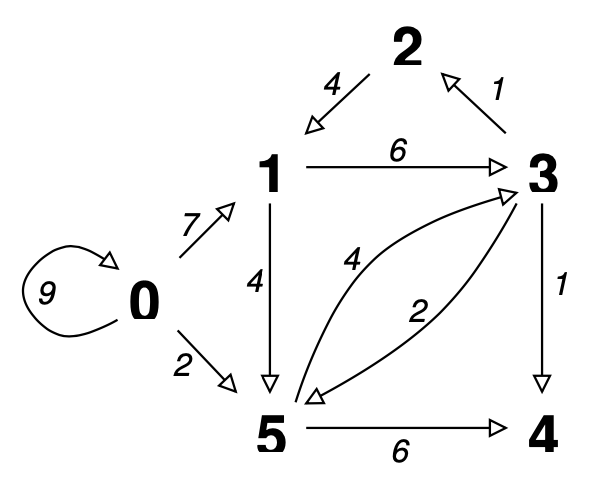
\includegraphics[width=3.5cm]{images/esempio-grafo-pesato.png}
        \caption{}
    \end{subfigure}
    \hfill
    \begin{subfigure}{.3\textwidth}
        \centering
        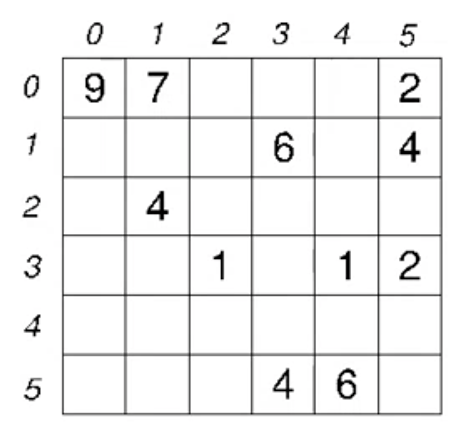
\includegraphics[width=3.5cm]{images/matrice-adiacenza-pesata.png}
        \caption{}
    \end{subfigure}
    \hfill
    \begin{subfigure}{.3\textwidth}
        \centering
        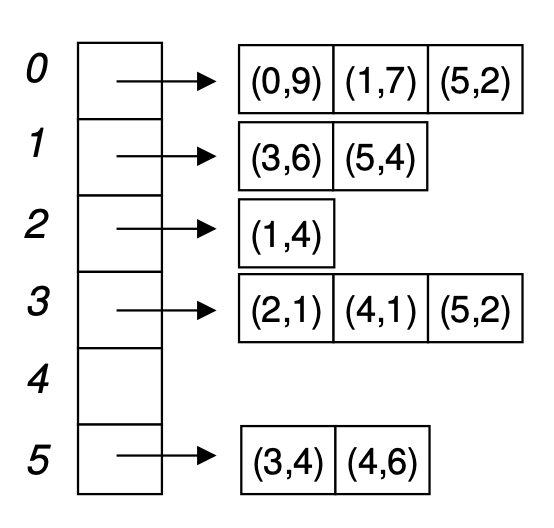
\includegraphics[width=3.5cm]{images/lista-adiacenza-pesata.png}
        \caption{}
    \end{subfigure}
    \vspace{-5pt}
    \caption{In (a) il grafo pesato, in (b) la matrice pesata ed in (c) la lista pesata}
\end{figure}

\newpage
\subsection{Cammini}
\begin{definition}[Cammino]
    Un \textbf{cammino} è una sequenza di nodi collegati da archi (nella stessa direzione).
\end{definition}

\subsubsection{Walk, trail e path}
Esistono 3 tipi di cammini: il \textbf{walk}, il \textbf{trail} ed il \textbf{path}
\begin{definition}[Walk]
    Dato un grafo orientato $G = (V,E)$ un \textbf{walk} è una sequenza di nodi.
    \begin{center}
        $P = v_0, v_1, \ldots, v_k$ tale che $(v_i,v_{i+1}) \in E$ per ogni $i \in K$
    \end{center}
\end{definition}
\hspace{-15pt}Vediamo che la \textbf{lunghezza} di $P$ è uguale a $k$ mentre gli estremi di un walk $P$ sono $v_0$ e $v_k$, e si dice che $P$ inizia con $v_0$ e termina con $v_k$.
\begin{note}
Un walk di lunghezza $0$ è un semplice nodo.
\end{note}

\begin{definition}[Trail e path]
    Un walk $P$ è detto \textbf{trail} se attraversa ogni arco in $E$ al più una volta. Un trail è detto \textbf{path} se attraversa ogni nodo in $V$ al più una volta.
\end{definition}

\begin{example}
    Prendendo come esempio l'immagine \ref{fig:esempio-grafo} vediamo che:
    \begin{itemize}
        \item La sequenza $\{0, 0, 1, 3, 2, 1, 3, 2\}$ è un walk ma non è un trail.
        \item Mentre la sequenza $\{0, 0, 1, 3, 4, 3, 4\}$ è un trail ma non è un path.
        \item Infine la sequenza $\{0, 1, 3, 4\}$ è un path.
    \end{itemize}
\end{example}

\subsubsection{Enunciati sui cammini}
\begin{proposition}\label{proposizione-walk-1}
Sia $G = (V,E)$ un grafo orientato e siano $x,y \in V$ due nodi. Allora vale che:
\begin{center}
    \footnote{Ricorda che $E^n$ è una composizione di$ $E per $n$ volte, quindi con $n=3$ è $E;E;E$}Esiste un walk di lunghezza $n\in \mathbb{N}$ da $x$ a $y$ $\Longleftrightarrow (x,y) \in E^n$
\end{center}
\end{proposition}
\begin{demostration}
Dimostrammo la proposizione \ref{proposizione-walk-1} per induzione.
\begin{enumerate}
    \item \underline{Caso base:} con $n=0$ può esistere un solo walk di lunghezza 0 e sarebbe un walk $(x,x)$ con il nodo $x \in V$. Questo caso si dimostra facilmente visto che $E^0 = Id_E$ e per definizione di identità $(x,x) \in Id_E$.
    \item \underline{Passo induttivo:} Per ipotesi induttiva assumiamo che il caso per un walk di lunghezza $n$ sia vero, dimostriamo ora che vale anche quello di lunghezza $n+1$. \\ \\
    Noi sappiamo che esista un walk di lunghezza $n + 1$ fra $x$ e $y$:
    \begin{enumerate}
        \item $\Longleftrightarrow \: \exists$ un walk $x, v_1, v_2, ..., v_n, y$ che a sua volta esiste.
        \item $\Longleftrightarrow (x, v_1) \in E$ ed esiste un walk $v_1, v_2, ..., v_n, y$, che esiste.
        \item $\Longleftrightarrow (x, v_1) \in E$ e $(v_1,y) \in E^n$.
        \item $\Longleftrightarrow (x,y) \in E^{n+1}$
    \end{enumerate}
    Nel (c) il primo passaggio del walk deve esistere già in $E$ ($E$ senza ulteriori composizioni$E^n$), il resto del walk invece è $(v_1,y) \in E^n$ e non in $n+1$ perché avendo "tolto" e messo a se il primo passo ($(x, v_1) \in E$) ci rimane un cammino di lunghezza $n$. Se quindi facciamo la composizione fra $E$ ed $E^n$ ($E;E^n$) torna che è uguale a dire $E^{n+1}$, quindi arriviamo al punto (d) che dimostra il passo induttivo. $\blacksquare$
\end{enumerate}
\end{demostration}

\newpage
\begin{lemma}\label{lemma-1}
    Sia $G=(V,E)$ un grafo orientato e siano $x,y \in V$ due nodi. Allora vale che:
    \begin{enumerate}
        \item Se esiste un walk da x a y $\Longrightarrow$ esiste un trail da x a y.
        \item Se il walk ha lunghezza $>0$, allora anche il trail ha lunghezza $>0$.
    \end{enumerate}
\end{lemma}
\begin{demostration}
Questo lemma può essere dimostrato intuitivamente in entrabi i suoi punti. \\ \\
\underline{Caso 1:} Innanzitutto partiamo da un walk P = 1,2,3,4,1,2,6,5 dove c'è almeno una ripetizione dello stesso arco (in questo caso si passa 2 volte fra 1,2) che quindi non lo rende un trail.\\
Possiamo però rendere questo walk un trail rimuovendo tutti i collegamenti da una all'altra coppia ripetuta (in questo caso si rimuove "3,4,1,2") visto che se 2 è connesso a 6 possiamo connetterlo direttamente senza passare per 3,4,1,2. Eseguendo questa operazione per tutte le ripetizioni otteniamo un trail. \\\\
\underline{Caso 2:} Se esiste un walk di lunghezza maggiore di 0 fra $x$ e $y$, come visto sopra, esisterà anche un trail fra $x$ e $y$, ma è immediato dire che se esiste un trail fra questi due nodi deve esistere almeno un arco che li collega e che quindi dimostra che la lunghezza è $>0$.
$\blacksquare$
\end{demostration}
\begin{figure}[h!]
    \centering
    \begin{subfigure}{.3\textwidth}
        \centering
        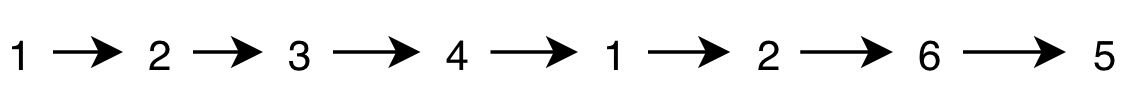
\includegraphics[width=5cm]{images/lemma-walk-trail-3.png}
        \caption{}
    \end{subfigure}
    \hfill
    \begin{subfigure}{.3\textwidth}
        \centering
        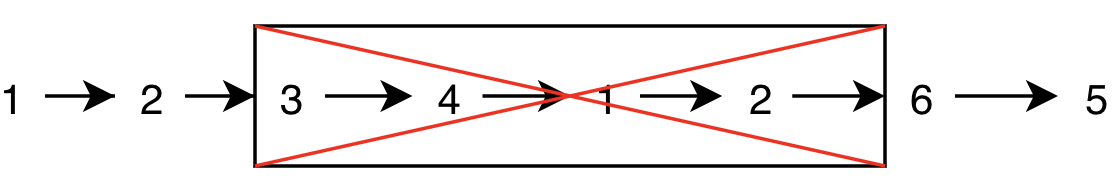
\includegraphics[width=5cm]{images/lemma-walk-trail-2.png}
        \caption{}
    \end{subfigure}
    \hfill
    \begin{subfigure}{.3\textwidth}
        \centering
        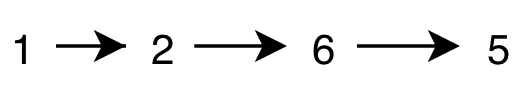
\includegraphics[width=3.5cm]{images/lemma-walk-trail-1.png}
        \caption{}
    \end{subfigure}
    \vspace{-5pt}
    \caption{Steps di trasformazione di un walk in un trail}
\end{figure}

\begin{lemma}\label{lemma-2}
Sia $G=(V,E)$ un grafo orientato e siano $x,y \in V$ due nodi. Allora vale che:
\begin{center}
    Se esiste un trail da x a y, allora esiste un path da x a y.
\end{center}
\end{lemma}
\begin{demostration}
Pure questo lemma si dimostra in maniera abbastanza intuitiva. Se prendiamo infatti un trail P = 4,5,6,7,6,9 che avendo una ripetizione di un nodo (il 6) non è un path, possiamo però farlo diventare andando a costruire un path rimuovendo il nodo ripetuto insieme a tutti i nodi intermedi (fra i due nodi doppi) e connettere il collegamento del nodo ripetuto al nodo mantenuto, riportato a questo esempio rimuoviamo 7,6 e connettiamo 9 a 4,5,6, questo fa uscire un path 4,5,6,9. Nel caso che con questa operazioni non sia ancora uscito un path basta ri-eseguirla per tutti i nodi ripetuti che rimangono. $\blacksquare$
\end{demostration}
\begin{figure}[h!]
    \centering
    \begin{subfigure}{.3\textwidth}
        \centering
        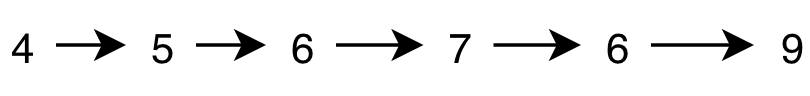
\includegraphics[width=5cm]{images/trail-path-1.png}
        \caption{}
    \end{subfigure}
    \hfill
    \begin{subfigure}{.3\textwidth}
        \centering
        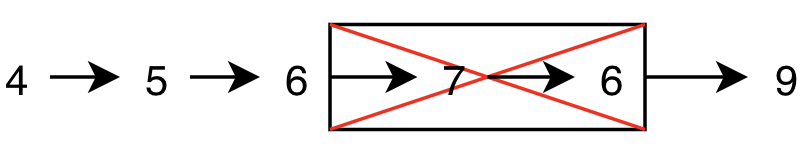
\includegraphics[width=5cm]{images/trail-path-2.png}
        \caption{}
    \end{subfigure}
    \hfill
    \begin{subfigure}{.3\textwidth}
        \centering
        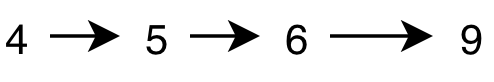
\includegraphics[width=3.5cm]{images/trail-path-3.png}
        \caption{}
    \end{subfigure}
    \vspace{-5pt}
    \caption{Steps di trasformazione di un trail in un path}
\end{figure}

\subsubsection{Walk chiusi, circuiti, cicli}
Quando in un walk si parte e si termina sullo stesso nodo possiamo andare a definire tale cammino in uno di questi 3 modi.
\begin{definition}[Walk chiuso, circuito e ciclo]\label{walk-chiusi-circuiti-cicli}
    Dato un walk P esso si definisce \textbf{walk chiuso} se gli estremi sono lo stesso nodo. Un walk chiuso che è un trail si definisce \textbf{circuito}, mentre un circuito che è un path viene chiamato \textbf{ciclo} (Senza considerare gli estremi).
\end{definition}
\begin{definition}[Grafo ciclico]
    Un grafo G si dice \textbf{ciclico} se esiste almeno un ciclo in G, in caso contrario di dice aciclico
\end{definition}

\newpage
\begin{proposition}\label{proposizione-walk-2}
    Sia G = (V,E) un grafo orientato e x un nodi in V. Le seguenti affermazioni sono equivalenti:
    \begin{enumerate}
        \item Esiste un walk chiuso da x a x.
        \item Esiste un circuito da x a x.
        \item Esiste un ciclo da x a x.
        \item $(x,x) \in E^*$
    \end{enumerate}
\end{proposition}
\begin{demostration}
Anche questa proposizione si dimostrazione intuitivamente applicando gli enunciati visti prima. Innanzitutto partiamo a dimostrare che se (1) allora (2). Questa affermazione è vera per la proposizione \ref{lemma-1}. Dimostriamo ora che se (2) allora (3). Questo si dimostra rapidamente come prima applicando una proposizione vista in precedenza, in questo caso la \ref{lemma-2}. In fine per la proposizione \ref{proposizione-walk-1} (1) se e solo se (4). E così dimostrato che queste 4 affermazioni si equivalgono. $\blacksquare$
\end{demostration}


\subsection{Connettività}
\begin{definition}[Fortemente connesso]\label{grafo-fortemente-connesso}
    Dato un grafo orientato $G = (V,E)$ si dice che questo grafo è \textbf{fortemente connesso} se per ogni coppia di nodi $x,y \in V$ esiste un walk da $x$ a $y$.
\end{definition}
\begin{definition}[Componente fortemente connesso]\label{componente-fortemente-connesso}
    Una componente fortemente connessa (SCC) di $G$ è un sottoinsieme non vuoto di nodi $U \subseteq V$ tale che:
    \begin{enumerate}
        \item Per ogni coppia di nodi $x,y \in U$ esiste un walk da $x$ a $y$.
        \item Se esiste un $U' \subseteq V$ che soddisfa la $1$ e $U \subseteq U'$, allora $U = U'$ \footnote{$U$ si definisce sottoinsieme massimale}.
    \end{enumerate}
\end{definition}
\begin{example}
    Prendiamo per esempio l'immagine \ref{fig:esempio-SCC}:
\end{example}
\begin{wrapfigure}[9]{l}{6cm}
    \vspace{-10pt}
    \centering
    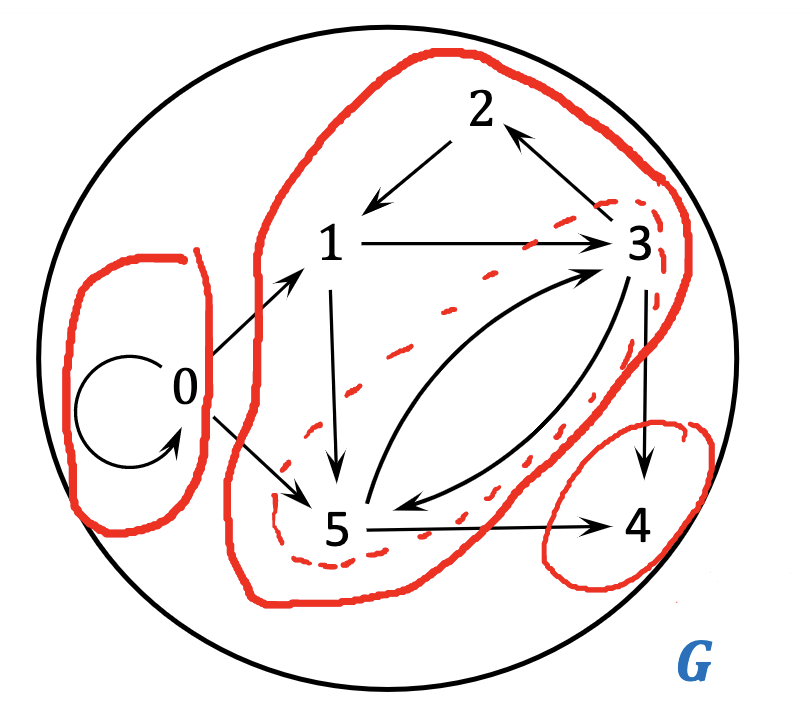
\includegraphics[width=3.7cm]{images/esempio-SCC.png}
    \caption{Grafo con i suoi SCC}
    \label{fig:esempio-SCC}
\end{wrapfigure}
In questa immagine vediamo che se prendiamo un sottoinsieme U = $\{5,4\}$ esso non è un SCC perchè non è validato il punto (2) visto che esiste un sottoinsieme $U' = \{1,3,5\}$ che lo contiene. \\Anche $U'$ non è un SCC mentre se prendiamo come $U = \{1,2,3,5\}$ questo è un SCC visto che c'è un walk per ogni elemento ed è il sottoinsieme massimale.\\
In questo esempio risulta che i SCC sono: 
\begin{center}
    $\{1,2,3,5\}$, $\{4\}$, $\{0\}$
\end{center}

\subsubsection{Componenti connesse e partizioni}
\begin{proposition}
    Dato un grafo $G=(V,E)$, l'insieme delle componenti fortemente connessi di $G$ è una partizione di $V$.
\end{proposition}
\begin{demostration}
Andiamo ora a dimostrare questa proposizione. Innanzitutto ricordiamo che $P = \{A_i\}_{i \in I}$ è una partizione dell'insieme $A$ se rispetta queste 3 condizioni:
\begin{enumerate}
    \item $\forall i$ $A_i \neq \O$
    \item $\bigcup^m_{i=1}A_j = A$
    \item $\forall i, j A_i \cap A_j = \O$ con $i \neq j$
\end{enumerate}
Quello che noi dobbiamo dimostrare è che l'insieme SCC = $\{C_1, C_2, \ldots, C_k\}$ è un partizione di $G$.
\begin{enumerate}
    \item La prima si dimostra immediatamente, perché un componente fortemente connesso non può essere vuoto per la sua definizione \ref{componente-fortemente-connesso}.
    \item Il secondo punto si dimostra prendendo una $x \in V$ e un insieme $U = \{x\}$, il quale rispetta la condizione (1) della definizione \ref{componente-fortemente-connesso}. Ora questo insieme può o essere una partizione, oppure esser contenuto in una componete fortemente connesso; capiamo dunque che se ripetiamo questa operazione per ogni elemento dell'insieme $V$ avremo una serie di SCC che alla peggio saranno tutti insiemi di un elemento o al meglio sarà tutto $V$, in ogni caso comunque ogni elemento apparterrà alla fine ad un SCC che se andiamo ad unire tutti insieme avremo $V$.
    \item Andiamo a dimostra il terzo punto per assurdo.\\ 
    Supponiamo che $\exists C_i, C_j$ partizioni distinte $\mid C_i \cap C_j \neq \O$. Se questa condizione è vera allora $\exists x \in C_i \cap C_j$ e $\exists y \in C_i \setminus C_j$ e anche $\exists z \in C_j \setminus C_i$ per definizione di intersezione.\\\\
    Se però la condizione che abbiamo posto per assurdo è vera allora $\forall \: y \in C_i$ e $\forall \: z \in C_j \Longrightarrow C_i \cup C_j$ soddisfa la proprietà (1) della definizione \ref{componente-fortemente-connesso}, e quindi che:\\
    $\exists$ walk $y \ldots x$, $\exists$ walk $x \ldots z \Longrightarrow \exists$ walk $y \ldots z$\\
    $\exists$ walk $z \ldots x$, $\exists$ walk $x \ldots y \Longrightarrow \exists$ walk $z \ldots y$ \\
    e questo dovrebbe avvenire perché se $C_i \cap C_j \neq \O$ vuol dire che c'è un elemento in comune in entrambi gli insieme che per la proprietà (1) dovrà avere un walk con gli altri elementi sia di $C_i$ che di $C_j$.
    Ma se ciò accadesse gli insiemi stessi $C_i$ e $C_j$ non sarebbero più partizioni perché sarebbe violata la proprietà (2) della definizione esistendo un insieme $C_i \cup C_j$ che li contiene. $\blacksquare$
\end{enumerate}
\end{demostration}

\subsubsection{Proprietà connettività}
\begin{proposition}\label{proposizione-connettività-1}
    Per tutti i grafi orientati $G=(V,E)$ e tutti gli $x,y \in V$ vale che:
    \begin{enumerate}
        \item $G$ è fortemente connesso $\Longleftrightarrow V \times V \subseteq E^*$.
        \item $(x,y) \in E^* \cap (E^*)^{op} \Longleftrightarrow$ $x$ ed $y$ appartengono alla stessa componente fortemente connessa.
    \end{enumerate}
\end{proposition}
\begin{demostration} \label{dimostrazione-prop-1}
Questo due proprietà sono vere perché:
\begin{enumerate}
    \item Nella prima dire di avere un grafo fortemente connesso vuol dire avere un grafo che per ogni $x, y \in V \times V$ nodi esiste un walk fra essi, ma ciò e vero se e solo se (per la proposizione \ref{proposizione-walk-1}) per ogni $x, y \in V \times V$ val che  $(x,y) \in E^*$\footnote{Ricorda che la stella di kleene applica la chiusura transitiva per rendere appunto transitivo l'insieme, quindi applica una sequenza di composizioni, che è lo stesso di $E^n$}, ma se ogni $(x,y)$ appartengono sia a $V \times V$ che a $E^*$ possiamo scrivere che $V \times V \subseteq E^*$ (non il viceversa perché la stella di kleene include anche la proprietà riflessiva).
    \item Per dimostrare la seconda consideriamo che se esiste un walk fra $x$ e $y$ e viceversa vuol dire che $x$ e $y$ fanno parte della stessa componente fortemente connessa e quindi $(x,y) \in E^*$ per la dimostrazione vista sopra, e $(x,y) \in (E^*)^{op}$, e questo perché: se lo vediamo come $(x,y) \in (E^{op})^*$ (possibile per le proprietà della stella di kleene) quello che facciamo è andare ad invertire tutti gli archi in E e poi aggiungere la chiusura di kleene che, aggiungendo la proprietà transitiva all'insieme, fa si che esista un walk fra (x,y); quindi in conclusione visto che ($x,y$) apparitene ad entrambi gli insiemi apparterrà anche alla loro composizione $(x,y) \in E^* \cap (E^*)^{op}$. $\blacksquare$
\end{enumerate}
\end{demostration}

\subsection{Grafo orientato aciclico (DAGs)}
\begin{definition}[DAG, Sorgenti, Pozzi]
    Un grafo orientato senza cicli si chiama \textbf{Directed Acyclic Graph (DAG)}. Al suo interno possono esistere uno o più nodi di grado di ingresso $0$ detti \textbf{sorgenti} e uno o più nodi di grado di uscita $0$ detti \textbf{pozzi}
\end{definition}

\begin{proposition}
    Se $G = (V,E)$ è un DAG, allora $E^*$ è un ordinamento parziale.
\end{proposition}
\begin{demostration}
Per dimostrare che un grafo è un DAG, allora la stella di Kleene sugli archi ($E^*$) è un ordinamento parziale. Bisogna quindi dimostrare le 3 proprietà che rendono una relazione su un insieme un ordinamento parziale, e cioè la \textbf{transitività}, la \textbf{anti-simmetria} e la \textbf{riflessività}.
\begin{itemize}
    \item \underline{Dimostrazione \textbf{transitiva} e \textbf{riflessiva}}: Queste due proprietà si dimostrano velocemente visto che la stella di Kleene aggiunge sia la proprietà transitiva che riflessiva all'insieme.
    \item \underline{Dimostrazione \textbf{anti-simmetrica}}: Per dimostrare questa proprietà basta, per il punto (4) del teorema di caratterizzazione \ref{teorema-caratterizzazione}, andare a dimostrare che $E^* \cap (E^*)^{op} \subseteq Id_V$.\\
    Ora noi sappiamo che se $(x,y) \in E^* \cap (E^*)^{op}$ esiste un walk fra $x$ e $y$ e viceversa per la proposizione \ref{proposizione-walk-1} (questo perché come anche descritto nella dimostrazione \ref{dimostrazione-prop-1} la stella di Kleene aggiunge una concatenazione di composizioni). Se poniamo per assurdo che $x \neq y$ quello che risulterebbe sarebbe un walk chiuso che attraversa entrambi, perché se esiste un walk ($x,y$) ed uno ($y, x$) esso crea un ciclo, ma questo non può essere possibili perché abbiamo supposto per ipotesi che $G$ sia un DAG. Quindi risulta che $x = y$. $\blacksquare$
\end{itemize}
\end{demostration}

\subsubsection{Ordinamento topologico}
\begin{definition}
    Dato un DAG $G = (V,E)$ un ordinamento topologico di $G$ è una biiezione $\eta: V \to n$ con $n = \{0,1,2,\ldots, n-1\}$ \footnote{Si ricorda che per la definizione vista nel capitolo 1 ogni numero naturale $n$ denota un insieme}tale che:
    \begin{equation}
        \textbf{per ogni arco } (u,v) \in E \textbf{ vale } \eta(u) < \eta(v)
    \end{equation}
\end{definition}
\hspace{-15pt}In altre parole, se disponiamo i vertici lungo una linea orizzontale in base alla loro numerazione $\eta$, in ordine crescente, otteniamo che gli archi risultano tutti orientati da sinistra verso destra
\begin{proposition}
    Ogni DAG ha almeno un ordinamento topologico, e ne possono esistere di più.
\end{proposition}

\subsection{Grafo non orientato}
\begin{definition}[Grafo non orientato]
    Un grado non orientato $G = (V,E)$ ha un insieme finito di nodi $V$ e un insieme di archi $E = P_2(V)$ dove $P_2(V) = \{X \subseteq V \mid |X| = 2\}$
\end{definition}
\begin{wrapfigure}[8]{l}{6cm}
    \vspace{-15pt}
    \centering
    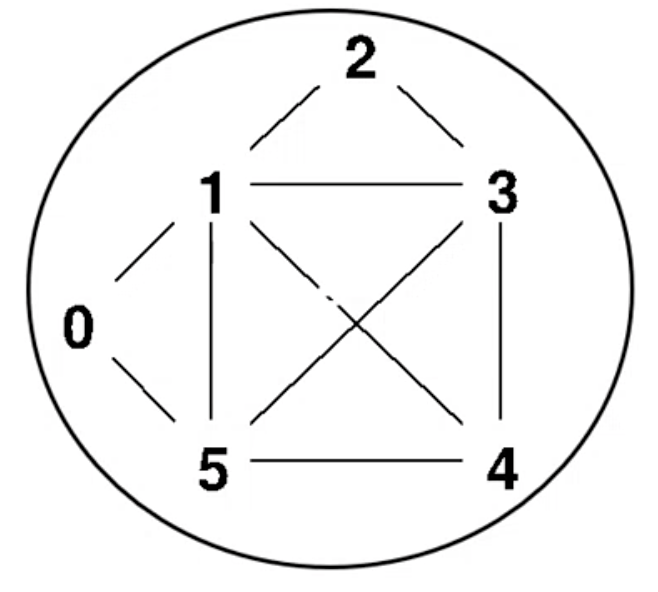
\includegraphics[width=3.7cm]{images/esempio-grafo-non-orientato.png}
    \vspace{-5pt}
    \caption{Grafo G non oriento}
    \label{fig:esempio-grafo-non-orientato}
\end{wrapfigure}
La caratteristica principale dei grafi non orientati è che gli archi non hanno una direzione, quindi sono sottoinsiemi di nodi di cardinalità $2$. Scriviamo un arco fra $x$ ed $y$ come $xy \in E$, ovvero $\{x,y\} \in E$. Un grafo orientato inoltre non può avere cappi.\\ \\
Quello in figura \ref{fig:esempio-grafo-non-orientato} è un esempio di grafo non orientato. \\\\\\\\
\textbf{Notazione.} Alcune definizioni e notazioni sui grafi non orientati. Dato un grafo $G = (V,E)$ non orientato si dice che:
\begin{itemize}
    \item Il \textbf{vicinato} di un nodo $x \in V$: \hspace{.7cm} $N(x) = \{y \in V \mid xy \in E\}$
    \item Il \textbf{grado} di un nodo $x \in V$: \hspace{.7cm} $d_x = \lvert N(x)\rvert$.
\end{itemize}
\begin{definition}[Universale, Isolato]
    Un nodo $x$ si dice Univalente se è vicino di tutti i nodi quindi $N(x) \cup \{x\} = V$, mentre un nodo si dice isolato se non ha vicinato, quindi $N(x) = \O$
\end{definition}

\begin{definition}[Grafo orientato associato]
    Dato un grafo non orientato $G = (V,E)$, quindi un grafo con $E \subseteq P_2(V)$, il \textbf{grafo orientato associato} a $G$ è il grafo orientato $\widetilde{G} = (V, \widetilde{E})$, dove la relazione $\widetilde{E}$ è definita come:
    \begin{center}
        $\widetilde{E} = \{(x,y) \in V \times V \mid \{x,y\} \in E\}: V \leftrightarrow V$
    \end{center}
\end{definition}

\begin{figure}[h!]
    \centering
    \begin{subfigure}{.3\textwidth}
        \centering
        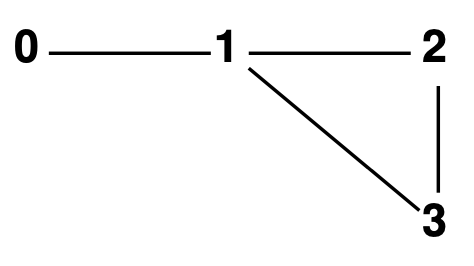
\includegraphics[width=3.5cm]{images/grafo-non-orientato.png}
        \vspace{-5pt}
        \caption{}
    \end{subfigure}
    \hspace{1cm}
    \begin{subfigure}{.3\textwidth}
        \centering
        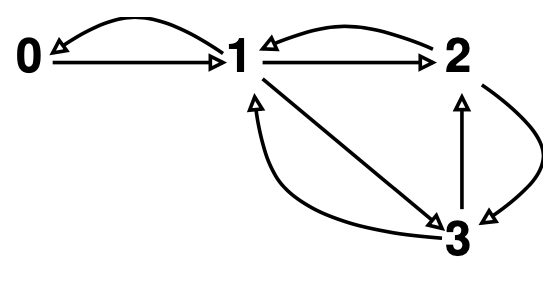
\includegraphics[width=3.5cm]{images/grafo-orientato-associato.png}
        \vspace{-5pt}
        \caption{}
    \end{subfigure}
    \caption{In (a) il grafo non orientato ed in (b) il rispettivo grafo non associato}
\end{figure}

\subsubsection{Hand-shaking lemma}
	L'hand-shaking lemma varia per i grafi non orientatati rispetto a come era definito per quelli orientati.
\begin{lemma}[Hand-shaking lemma]
    Per ogni grafo non orientato $G = (V,E)$, vale che:
    \begin{center}
        $\sum\limits_{x \in V}d_x = 2\lvert E\rvert$
    \end{center}
    Esso dice infatti che la somma dei gradi di tutti i nodi è uguale a $2$ volte il numero di archi del grafo. 
\end{lemma}
Il lemma è valido perché: osservando che con l'aggiunta di un arco in un grafo si va a incrementare di $1$ il grado di $2$ nodi differenti, visto che un arco dovrà per forza connettere due nodi che non possono essere lo stesso (non esistendo il cappio), aumenterà di $2$ volta la somma di tutti i gradi, mentre aumenterà solo di $1$ il numero di archi, avendo aggiunto un solo arco, basta dunque andare a moltiplicare per $2$ il numero di archi per ottenere la somma dei gradi.

\subsubsection{Rappresentazione grafi non orientati}
Le rappresentazioni per i grafi non orientati sono similari a quelle dei grafi orientati. Esiste infatti sia la rappresentazione tramite \textbf{matrice di adiacenza} che tramite \textbf{lista di adiacenza}; le uniche differenze sono che, non esistendo un verso per gli archi, verranno riscritti $2$ volte i collegamenti, uno per ogni direzione, questo sia nelle matrici che nelle liste.
\begin{figure}[h!]
    \centering
    \begin{subfigure}{.3\textwidth}
        \centering
        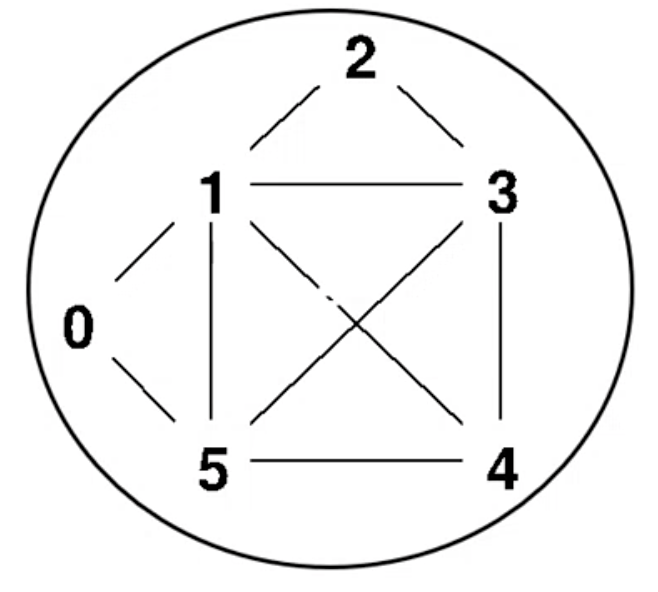
\includegraphics[width=3.3cm]{images/esempio-grafo-non-orientato.png}
        \caption{}
    \end{subfigure}
    \hfill
    \begin{subfigure}{.3\textwidth}
        \centering
        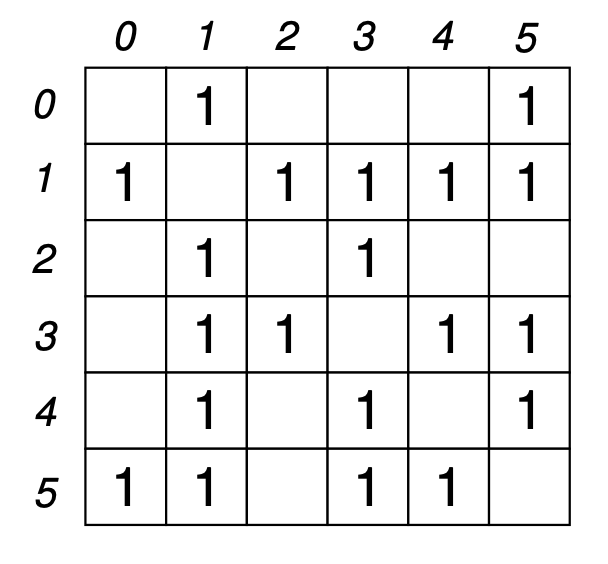
\includegraphics[width=3.3cm]{images/matrice-grafo-non-orientato.png}
        \caption{}
    \end{subfigure}
    \hfill
    \begin{subfigure}{.3\textwidth}
        \centering
        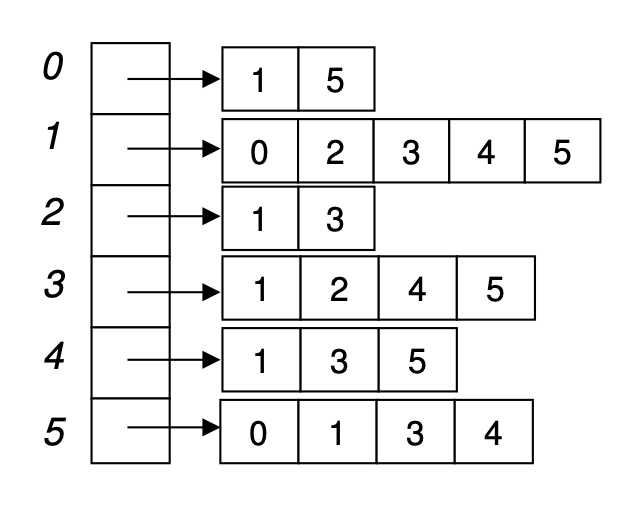
\includegraphics[width=3.3cm]{images/lista-grafo-non-orientato.png}
        \caption{}
    \end{subfigure}
    \vspace{-5pt}
    \caption{In (a) il grafo non orientato, in (b) la matrice ed in (c) la lista di adiacenza}
\end{figure}

\subsubsection{Cammini nei grafi non orientati}
\begin{definition}[Walk]
    In un grafo non orientato $G = (V,E)$, un walk è una sequenza di nodi
    \begin{center}
        $P = v_0, \ldots, v_k$ tale che $\{v_i, v_i+1\} \in E$ per ogni $i \in K$
    \end{center}
    La lunghezza del walk $P$ è uguale a $k$.
\end{definition}

\begin{definition}[Trail, path]
    Si definisce trail un walk che non attraversa due volte lo stesso arco. Un path è un walk (o trail) che non attraversa due volte lo stesso nodo.
\end{definition}

Le proposizioni \ref{proposizione-walk-1}, \ref{proposizione-walk-2} e i lemmi \ref{lemma-1}, \ref{lemma-2}  sono validi in ugual modo per i grafi non orientati, bisogna solo tenere in considerazione il fatto che in questo tipo di grafi gli archi non hanno verso (in pratica bisogna sostituire la $E$ con $\widetilde{E}$), le dimostrazioni sono similari.

\subsubsection{Cicli e connettività nei grafi non orientati}
Per i grafi non orientati le definizioni di \textbf{walk chiuso}, \textbf{circuiti} e \textbf{cicli} sono uguali a quelli visti nei grafi orientati (Definizione \ref{walk-chiusi-circuiti-cicli}).
\begin{note}
Un walk chiuso (da $x$ a $x$) non implica un circuito (da $x$ a $x$), ma un circuito implica un ciclo
\end{note}
Ugualmente le definizioni di grafo \textbf{fortemente connesso} e  di \textbf{componente fortemente connesso} sono analoghe a quelle viste per i grafi orientati (Definizioni \ref{grafo-fortemente-connesso}, \ref{componente-fortemente-connesso}).\\
Anche qui, la proposizione \ref{proposizione-connettività-1} vale  per i grafi non orientati (bisogna sostituire la $E$ con $\widetilde{E}$).


\subsection{Cammini Euleriani}
\begin{definition}[Circuito e trail euleriano]
    Dato un grafo non orientato connesso $G = (V,E)$, un \textbf{circuito euleriano} è un circuito che passa esattamente una volta per tutti gli archi del grafo. Analogamente un \textbf{trail euleriano}. (conosciuto anche come percorso euleriano)
\end{definition}
Questa definizione parte del problema dei sette ponti di Konigsberg.
\begin{theorem}[Il teorema di Eulero]
Dato un grafo $G = (V,E)$ non orientato e connesso:
\begin{enumerate}
    \item Esiste un circuito euleriano $\Longleftrightarrow$ tutti i nodi hanno grado pari.
    \item Esiste un trail euleriano da $x$ a $y$, con $x \neq Y$ $\Longleftrightarrow$ $x$ a $y$ sono gli unici nodi di grado dispari.
\end{enumerate}
\end{theorem}

\begin{demostration}
Dimostrazione dei due punti del teorema di Eulero.\\\\
\underline{Punto (1)}: Per andare a dimostrare questo punto dobbiamo dimostrare i due sensi della freccia.
\begin{itemize}
    \item Se esiste un circuito euleriano $\Longrightarrow$ tutti i nodi hanno grado pari.\\
    Questo caso è facilmente dimostrabile perché: possiamo notare che ogni volta che in un circuito euleriano noi passiamo per un nodo ($x \to y \to z$) attraversiamo $2$ archi mai attraversati, questo vuol dire che il numero di archi incidenti\footnote{Ricorda che gli archi incidenti sono gli archi che escono/entrano in un nodo, in un grafo non orientato} in un nodo è il doppio delle volte in cui il circuito ci passa, inoltre non può verificarsi una casistica in cui un nodo ha solo un arco perché in quel modo non ci verificherebbe un circuito.\\ Essendo che il numero di archi incidenti ad un nodo è il doppio non potrà mai essere un numero dispari.
    \item Se tutti i nodi hanno grado pari $\Longrightarrow$ esiste un circuito euleriano.\\
    Innanzitutto prendiamo un nodo $r$ ed iniziamo a creare un percorso in G marcando ogni arco in cui passiamo in modo da non passarci una seconda volta, a questo punto solamente $r$ avrà un solo arco incidente marcato all'inizio, mentre ogni nodo in cui passiamo avrà due archi marcati (un per arrivarci ed uno per andare), continueremo finché non ritorneremo nel nodo $r$ creando un circuito, non potrà essere altrimenti perché se il nodo finale $u \neq r$ allora vorrebbe dire che ha un numero di archi incidenti dispari (avendo un arco per arrivarci e non uno per uscirci) e questo non è possibile per ipotesi.\\\\
    A questo punto chiamiamo il circuito trovato C, se C passa per tutti gli archi allora è euleriano ed abbiamo finito, in caso contrario dobbiamo utilizziamo l'ipotesi che G sia connesso per così dedurre che esista un nodo $r'$ in C che ha un arco incidente non marcato.\\\\ 
    Prendiamo ora $r'$ e ripetiamo l'operazione vista prima andando a ricreare un nuovo circuito $C'$, notiamo che $C'$ e $C$ sono disgiunti sugli archi (perché marchiamo man mano gli archi che passiamo), inoltre $C$ e $C'$ si incontreranno in $r'$. \\\\
    A questo punto avremo due circuiti $C$ e $C'$ che coincidono in un nodo $r'$ e con tutti archi disgiunti, se quindi andiamo ad unire questi due circuiti prendendo come nodo di partenza e di arrivo $r'$ avremo un circuito che o è euleriano o avrà un nodo $r''$ con un arco non segnato, vediamo dunque che possiamo nuovamente ripetere l'operazione precedentemente vista altre $n$ volte, andando volta in volta a combinare i circuiti trovati fino a che non si creerà un circuito euleriano. $\blacksquare$
\end{itemize}
\underline{Punto (2)}: Anche qui bisogna dimostrare i due sensi della freccia per dimostrare la sua veridicità.
\begin{itemize}
    \item Se esiste un trail euleriano da $x$ a $y$, con $x\neq y \Longrightarrow$ $x$ e $y$ sono gli unici nodi di grado dispari.\\
    Questo verso lo dimostriamo vedendo che ogni volta che attraverso un nodo $v$ utilizzo $2$ archi, uno per entrare ed uno per uscire, le uniche eccezioni sono per il nodo di partenza e per quello di arrivo che avranno grado uguale a $2k + 1$ dove $k$ è il numero di volte in cui si passa per quel nodo (esclusa la partenza o l'arrivo) ed il $+1$ indica appunto la partenza nel caso di $x$ e l'arrivo nel caso di $y$. Abbiamo così dimostrato il primo verso.
    \item Se $x$ e $y$ sono gli unici nodi di grado dispari $\Longrightarrow $ esiste un trail euleriano da $x$ a $y$.\\
    Prendiamo per dimostrare questo caso un grado G = (V,E) che sua un grado connesso con $x,y \in V$ di grado dispari e $\forall v \in V . v\notin \{x,y\}$ siano di grado pari (queste condizioni sono vere per l'ipotesi).\\
    Ora creiamo un nuovo grafo $G'$ uguale a G solo introducendo un nuovo nodo $z$ con due archi $\{z,x\}$ e $\{z,y\}$ (questo nuovo nodo rispetta le condizioni poste nell'ipotesi). \\
    $G'$ è connesso visto che il nodo $z$ è connesso ad almeno un nodo il quale, appartenendo anche al grafo G che era connesso per ipotesi, è collegabile a tutti gli altri nodi, dunque che $z$ lo sarà, e quindi $G'$ è connesso.\\
    Essendo che $G'$ + connesso tutti, tutti i odi hanno grado pari $\exists$ circuito euleriano per il punto (1) di questo teorema. Ma visto che esiste un circuito euleriano $z,x,\ldots,y,z$ esisterà allora un trail $x,..,y$ che sarà euleriano nel caso si consideri il grafo $G$ (quindi senza $z$ e i suoi archi). Così dimostriamo anche questa implicazione. $\blacksquare$
\end{itemize}
\end{demostration}

\subsection{Cicli e path Hamiltoniani}
\begin{definition}[Cicli e path Hamiltoniani]
    Dato un grafo connesso (orientato o non orientato), un \textbf{ciclo hamiltoniano} è un ciclo che passa esattamente una volta per tutti i nodi del grafo. Analogamente, path hamiltoniano.
\end{definition}
Questo tipo di cammino non prevede una caratterizzazione semplice come per i circuiti euleriani. Equivale inoltre a cercare una permutazione dei nodi che formano un path.

\subsubsection{Il problema del commesso viaggiatore}
Il problema del commesso viaggiatore consiste, dato un grafo pesato non orientato, di trovare un ciclo hamiltoniano di peso minimo, dove il peso è la somma dei pesi degli archi attraversati.
\begin{figure}[h!]
    \centering
    \begin{subfigure}{.3\textwidth}
        \centering
        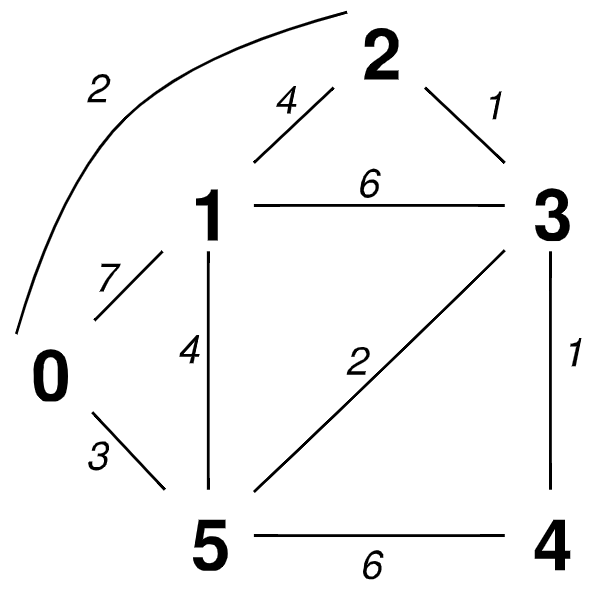
\includegraphics[width=3.3cm]{images/es-problema-viaggiatore-1.png}
        \caption{}
    \end{subfigure}
    \hfill
    \begin{subfigure}{.3\textwidth}
        \centering
        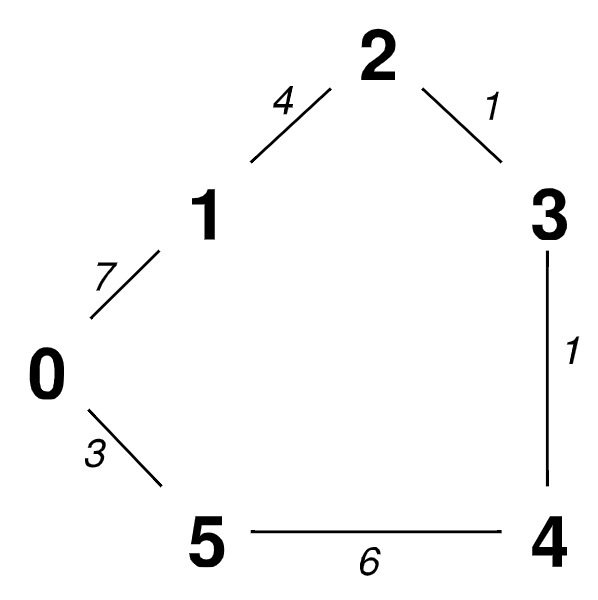
\includegraphics[width=3.3cm]{images/es-problema-viaggiatore-2.png}
        \caption{}
    \end{subfigure}
    \hfill
    \begin{subfigure}{.3\textwidth}
        \centering
        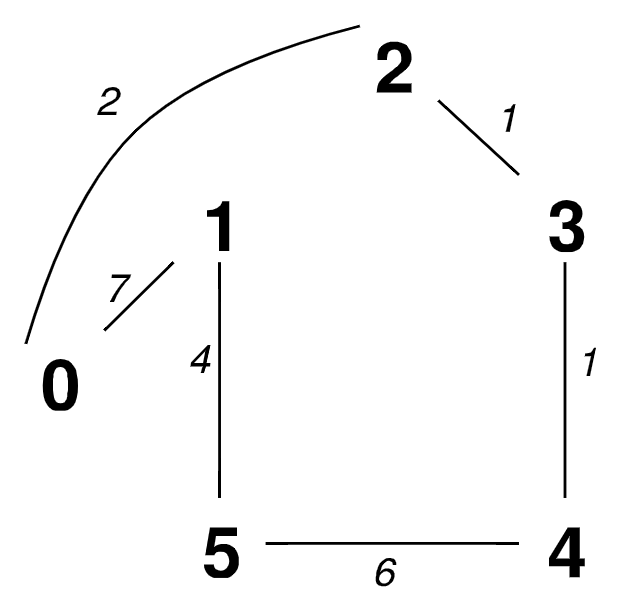
\includegraphics[width=3.3cm]{images/es-problema-viaggiatore-3.png}
        \caption{}
    \end{subfigure}
    \caption{(a) il grafo pesato, (b) ciclo hamiltoniano in (c) un ciclo hamiltoniano di peso minimo}
\end{figure}

\subsection{Distanze}
\begin{definition}[Distanza]
    Una \textbf{distanza} (o metrica) su un insieme A è una funzione $d: A \times A \to \mathbb{R}$ che soddisfa le seguenti proprietà per ogni $x,y,z \in A$.
    \begin{enumerate}
        \item $d(x,y) \geq 0$.
        \item $d(x,y) = 0 \Longleftrightarrow x = y$.
        \item $d(x,y) = d(y,x)$ (simmetria).
        \item $d(x,y) \leq (x,z) + d(z,y)$ (disuguaglianza triangolare)
    \end{enumerate}
\end{definition}
Si può notare che tutte queste condizioni sono soddisfatte dalla distanza euclidea \footnote{Ricorda che la distanza euclidea è la distanza fra due punti in un piano cartesiano}, infatti (1) la distanza euclidea è sempre maggiore o uguale a 0, e se è 0 è perché abbiamo preso due punti uguali (2), inoltre (3) la distanza fra due elementi non cambia, indipendentemente da quale punto prendiamo per prima, ed in fine in un triangolo la somma delle lunghezze di due lati  maggiore o uguale a quella del terzo lato (4).

\begin{definition}[Distanza su un grafo non orientato]
    Sia $G = (V,E)$ un grafo non orientato connesso. Dati due nodi $x,y \in V$, la loro \textbf{distanza} $d(x,y)$ è la lunghezza del walk più breve tra $x$ e $y$ (il cammino minimo).
\end{definition}
Possiamo vedere che in quest'ultima definizione sono rispettate i quattro punti della definizione di distanza.
\begin{enumerate}
    \item La distanza fra $x$ e $y$ è sempre $\geq 0$ perché in caso contrario vorrebbe dire che non esiste, e ciò non è possibile per la definizione stessa (nella definizione diciamo che il grafo è connesso).
    \item Se la distanza fra due nodi è $0$ allora il nodo è lo stesso.
    \item Se esiste un cammino da $x$ a $y$ con una certa distanza, questo cammino può essere percorso anche da $y$ a $x$ e quindi mantiene la stessa distanza.
    \item Essendo la distanza la lunghezza del walk più breve la distanza fra $x$ e $y$ sarà per forza minore o uguale di quella fra $x$ e $z$ sommata con quella fra $z$ e $y$.
\end{enumerate}

\begin{definition}[Distanza su grafo induttivamente]
    Sia $G = (V,E)$ un grafo non orientato connesso. Dati due nodi $x,y \in V$, al loro distanza $d(x,y)$ può essere definita induttivamente:
    \begin{itemize}
        \item \underline{Caso base}: $d(x,y) = 0$, se $x = y$.
        \item \underline{Passo induttivo}: $d(x,y) = 1 + min\{d(z,y) \mid z\in N(x)\}$. Dove $N(x)$ è il vicinato di $x$
    \end{itemize}
\end{definition}

La definizione di distanza (come lunghezza del cammino minimo) si può applicare anche a grafi orientati fortemente connessi, ma in questo caso non vengono rispettate tutte le proprietà:
\begin{enumerate}
    \item $d(x,y) \geq 0$ è vera per la definizione di grafo fortemente connesso.
    \item $d(x,y) = 0$ se e solo se $x = y$ è vera perché l'unico cammino di lunghezza $0$ è quello fra un nodo e se stesso.
    \item $d(x,y) = d(y,x)$ invece non è rispetta perché essendoci un verso negli archi possono esistere percorsi più brevi differenti.
    \item Visto che il punto (3) non è verificato non è necessario verificare il (4).
\end{enumerate}
Nel caso di grafi fortemente orientati definiamo la funzione della distanza una quasi-metrica.

\begin{proposition}\label{proposizione-distanza-1}
    Sia $G = (V,E)$ un grafo orientato connesso e $x$ un nodo. Sia $y$ un nodo a distanza massima da $x$, allora $G\setminus \{y\}$ è connesso.
\end{proposition}

\begin{demostration}
    Dimostriamo la proposizione scritta sopra, essa dice che:
    \begin{center}
        $\forall v \in V, d(x,y) \geq d(x,v) \Longrightarrow \forall v \in V \setminus \{y\}$ $\exists$ path $P = x,\ldots,v$. che non include y.
    \end{center}
    I path $P = x,\ldots,v$ non devono includere y perché se lo includesse allora $\exists$ $P' = x\ldots,y$ più corto di $P$ e questo contraddice che $d(x,y) \geq d(x,v)$.\\
    Se dal nostro grafo rimuovo y segue per quanto detto prima che $\forall v \in V \setminus \{y\}$ esiste ancora un path $P = x,\ldots,v$.
    Allora vediamo che $\forall v,w$ $\exists$ walk $W = v,\ldots,x,\ldots,w \Longrightarrow G \setminus \{y\}$ è connesso. $\blacksquare$
\end{demostration}

\subsubsection{Diametro, altezza, profondità}
\begin{definition}[Diametro di grafo]
    Il diametro di un grafo $G$ (oriento o meno) è la massima distanza tra coppie di nodi:
    \[diam(g) = \max_{x,y \in V}d(x,y)\]
\end{definition}

\begin{definition}[Profondità, altezza di nodi, albero pieno]
    Dato un albero radicato, la \textbf{profondità} di un nodo $x$ è la distanza $d(x,t)$ dalla radice $r$, e \textbf{l'altezza} di $x$ è la massima distanza tra $x$ e le sue foglie discendenti. L'altezza dell'albero è l'altezza della radice. Inoltre definiamo un albero cardinale come \textbf{pieno} se è completo e le foglie sono tutte alla stessa distanza dalla radice.
\end{definition}



\newpage
\subsection{Alberi}

\begin{definition}[Albero, foglia]
    Un \textbf{albero} è un grafo non orientato connesso, aciclico e non vuoto (con almeno $1$ nodo).
    I nodi interni hanno quindi grado $>1$ mentre i nodi di grado $1$ sono detti \textbf{foglie}.
\end{definition}

\begin{definition}[Foresta]
    Una \textbf{foresta} è un grafo non orientato, aciclico e non vuoto dove ogni componente connessa è un albero assestante.
\end{definition}
\hspace{-15pt}Da queste definizioni possiamo dedurre alcune proprietà relative agli alberi.
\begin{wrapfigure}[8]{r}{7cm}
    \centering
    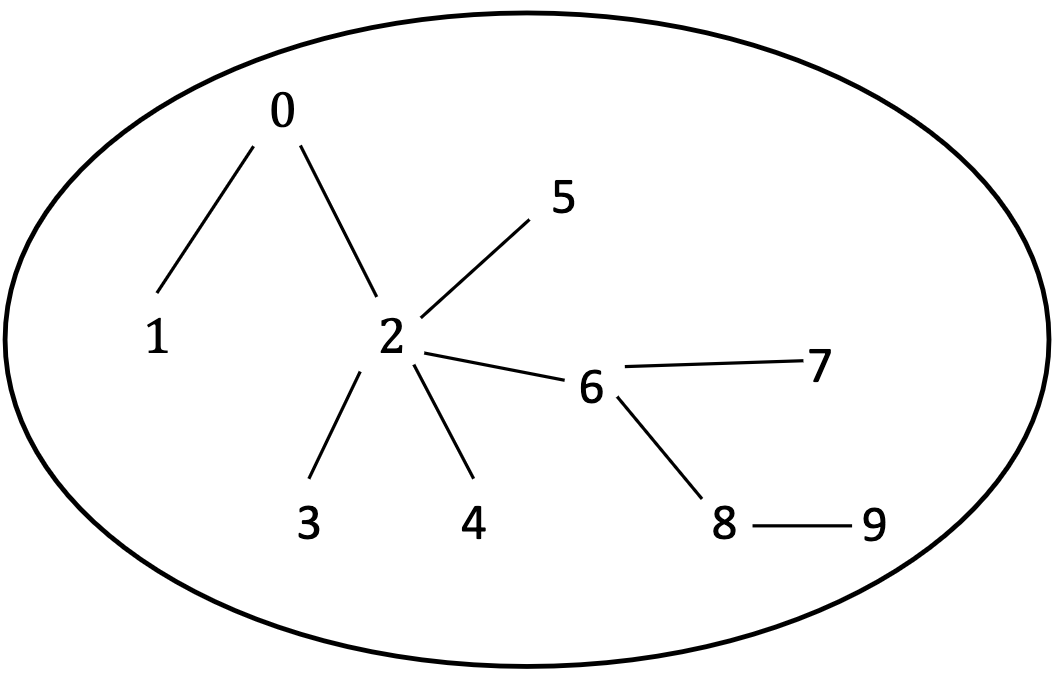
\includegraphics[width=5cm]{images/es-albero.png}
    \vspace{-5pt}
    \caption{Esempio di albero}
\end{wrapfigure}
\begin{itemize}
    \item Il numero di path possibili fra due nodi è sempre uno, perché se esistessero due path distinti la concatenazione di questi due path sarebbe un walk chiuso e quindi il grafo avrebbe cicli (ricorda la proposizioni \ref{proposizione-walk-2} che ci dice che dire walk chiuso o ciclo è analogo).
\end{itemize}

\begin{itemize}
    \item Se andiamo a toglie un arco in un albero si andrà a creare una foresta con 2 alberi.
    \item Se invece andiamo ad aggiungere un arco quello che uscirà non sarà più un albero perché si creerà un ciclo.
\end{itemize}


\begin{proposition}
    Dato un albero G = (V,E) con $n = |V|$ nodi, valgono le seguenti proprietà:
    \begin{enumerate}
        \item Se $n \geq 2$ (ovvero l'albero ha almeno due nodi), allora G ha almeno una foglia (ovvero un nodo di grado 1).
        \item G ha esattamente $n-1$ archi, cioè $|E| = n-1$.
        \item Per ogni coppia di nodi distinti $x,y \in V$, esiste un unico path da x a y.
        \item Per ogni arco $xy \in E$, la rimozione di $xy$ rende il grafo non connesso.
        \item Per ogni coppia di nodi distinti $x,y \in V$ tale che $xy \notin E$, l'aggiunta dell'arco xy crea un ciclo, cioè $G' = (V, E \cup {xy})$ è un ciclo.
    \end{enumerate}
\end{proposition}


\begin{demostration}
Andiamo ora a dimostrare ogni punto della proposizione sopra.
\begin{enumerate}
    \item Per dimostrare il primo punto prendiamo innanzitutto un albero T = (V,E) con almeno 2 nodi, per la proposizione \ref{proposizione-distanza-1} $\exists y \in V \: |\: T \setminus \{y\}$ è connesso $\Longrightarrow T \setminus \{y\}$ rimane connesso quindi rimane un albero.\\
    Ora, se re-introduciamo y possiamo vedere 2 casi:
    \begin{itemize}
        \item O $|N(y)| = 1$ (il vicinato di $y$ è 1), quindi $y$ è una foglia di T e la proprietà e verificata.
        \item Oppure $|N(y)| \geq 2$ (il vicinato di $y$ è maggiore o uguale a 2), in questo caso però $\exists$ path $P = w,...,z$ in $T \setminus \{y\}$ e $\exists \{z,y\}, \{y,w\} \in E$ (queste due condizioni sono previste visto che un albero è connesso), ma ciò porterebbe ad un ciclo che è impossibile.
    \end{itemize}
    Vediamo dunque che solo la prima casistica è possibile, e quindi abbiamo dimostrato questo punto. $\blacksquare$
    \item Per andare a dimostrare questo punto procediamo per induzione su n.
    \begin{itemize}
        \item \underline{Caso base:} Se n=1 allora l'albero ha un solo nodo e quindi nessun arco, la proprietà in questo caso è quindi dimostrate perché $n-1 = 0$, e $m=0$.
        \item \underline{Passo induttivo:} Assumiamo per ipotesi induttiva che la proprietà valga per tutti gli $n$ nodi, dimostriamo che vale anche per gli $n+1$ nodi. Un albero in questo caso ha almeno 1 nodo quindi $n \geq 1$ mentre nel caso $n+1$ gli alberi avranno come minimo 2 nodi ($n+1 > 1$ che è uguale a dire $n + 1 \geq 2$), per la proprietà (1) G ha almeno una foglia $y$.\\\\
        Prendiamo ora un albero $G' = G \setminus \{y\}$, togliamo dunque una foglia ed un arco (l'unico arco connesso a $y$) ed otteniamo che in $G'$ il numero di nodi $n = (n + 1)-1$ che quindi è $n = n$ ed il numero di archi è $m = (n-1)-1$ quindi $m = n$. Visto che $G'$ ha $n$ archi e $G$ ne ha $n+1$ abbiamo dimostrato l'ipotesi induttiva. $\blacksquare$
    \end{itemize}
    \item Dimostriamo questa proprietà per assurdo, quindi supponiamo che esistano due path distinsi $P_1$ e $P_2$ da $x$ a $y$. \\
    Prendiamo un nodo $z$ che sia l'ultimo nodo in comune fra $P_1$ e $P_2$ prima che $P_1$ e $P_2$ divergano in due percorsi distinti, e prendiamo un $w$ che sia invece il primo nodo dopo $z$ in $P_1$ attraversato anche da $P_2$ (l'esistenza di questi due nodi è obbligatoria perché $P_1$ e $P_2$ partono ed arrivano sugli stessi nodi, alla peggio $z = x$ e $w = y$). \\\\
    Essendo un albero un grafo connesso esisterà un cammino fra $z$ e $w$ che però sarà un ciclo perché partendo da $z$ andiamo a $w$ passando per i nodi di $P_1$ e da $w$ posso tornare a $z$ per i nodi in $P_2$; questa però è una contraddizione, è quindi verificata la proprietà. $\blacksquare$ 
    \item Questa propria si dimostra in modo veloce vedendo innanzitutto che se prendiamo un albero G con al suo interno due nodi $x$ e $y$ esisterà un unico path $P = xy$, perché in caso c'è ne fossero di più l'albero avrebbe un ciclo e quindi non sarebbe più un albero (meno di un path non è possibile per definizione di albero). Se andiamo a rimuovere P allora $\nexists$ path fra $x$ e $y$ e quindi il grafo non è connesso. $\blacksquare$
    \item Anche l'ultima proprietà si dimostra velocemente, visto che se abbiamo un albero G con due nodi $x$ e $y$ allora per definizione di albero $\exists$ path $P = x...y$ (che non sarà $xy$ per ipotesi), se aggiungiamo un arco $xy$ allora si otterrà un ciclo. $\blacksquare$
\end{enumerate}
\end{demostration}

\subsubsection{Albero radicato}
\begin{definition}[Albero radicato]
    Un \textbf{albero radicato} G=(V,E,r) è costituto da un albero G=(V,E) e da un nodo $r\in V$ chiamato \textbf{radice}.
\end{definition}

\begin{definition}[Antenato, genitore, discendete, figlio]
    Dato un albero radicato G=(V,E,r) e dato un nodo $y \in V$ e $y \neq r$ possiamo dare le seguenti definizioni.
    \begin{itemize}
        \item I nodi lungo l'unico cammino che collega y a r si chiamano \textbf{antenati}.
        \item Il primo nodo fra gli antenati (quello adiacente a y) è detto il \textbf{genitore} di y.
        \item Simmetricamente y viene detto \textbf{discendente} dei suoi antenati e \textbf{figlio} del nodo genitore.
    \end{itemize}
\end{definition}

\begin{definition}[Sottoalbero]
    Dato un albero radicato G = (V,E,r) e dato un nodo $r' \in V$ il \textbf{sottoalbero} di G con radice $r'$ è l'albero radicato G' = (V',E',r') in cui $V' \subseteq V$ contiene r' e tutti i suoi discendenti in G, e $E' \subseteq E$ contiene tutti gli archi di G tra i nodi di V'.
\end{definition}

\begin{wrapfigure}[9]{l}{7.5cm}
    \vspace{-15pt}
    \centering
    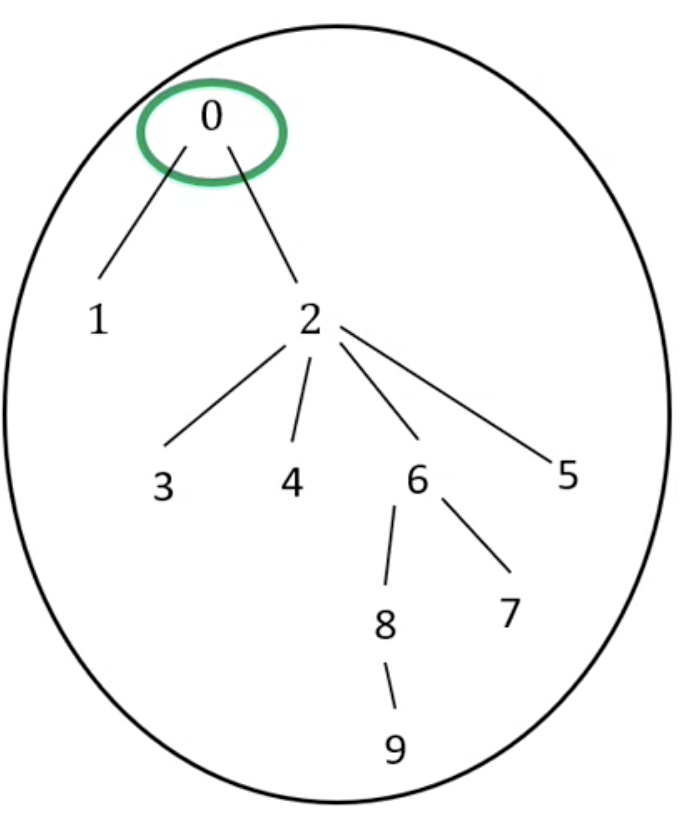
\includegraphics[width=3cm]{images/es-albero-radicato.png}
    \caption{Albero radicato con radice r}
    \label{es-albero-radicato}
\end{wrapfigure}

Se prendiamo l'immagine \ref{es-albero-radicato} vediamo che la radice $r = 0$.
La radice ha come figli 1 e 2 mentre 2 ha come antenato solo la radice.\\\\
Se prendiamo il nodo 8 questo nodo è padre di 9 e ha come fratello 7.\\
Il nodo 9 invece è un discendete di 2 essendo che 2 è un suo antenato.\\\\

\begin{definition}[Albero ordinale, albero cardinale]
    Un albero radicato si dice \textbf{albero ordinale} se per ciuscun nodo interno è definito un ordinamento totale tra i suoi figli. Un albero radicato si dice \textbf{albero cardinale} o k-ario se ogni nodo interno ha esattamente k figli, alcuni dei quali possono essere vuoti.
\end{definition}

\begin{definition}[Albero completo, binario]
    Un albero cardinale è \textbf{completo} se ogni nodo interno ha tutti e k i figli non vuoti. Un caso speciale di albero cardinale è quello con k=2, esso si dice infatti \textbf{albero binario}; in esso il primo figlio viene chiamato figlio sinistro ed il secondo figlio viene chiamato figlio destro.
\end{definition}

\subsection{Isomorfismo}
\begin{definition}[Isomorfismo]
    Dati due qualunque grafi $G_1 = (V_1, E_1)$ e $G_2 = (V_2, E_2)$ dove $\lvert V_1\rvert = \lvert V_2\rvert$ e $\lvert E_1\rvert = \lvert E_2\rvert$, un isomorfismo fra questi due  grafi è una biiezione $f: V_1 \mapsto V_2$ tra i loro nodi tale che:
    \begin{center}
        \vspace{-5pt}
        $\forall u,v \in V_1$ vale che $uv \in E_1 \Longleftrightarrow f(u)f(v) \in E_2$.
    \end{center}
\end{definition}
\hspace{-15pt}Possiamo definire due grafi isomorfi se esiste un isomorfismo fra di loro. Essere isomorfi è una relazione di equivalenza visto che sono presenti le proprietà riflessiva, simmetrica, transitiva.\\\\
Intuitivamente due grafi sono isomorfi se posso renderli identici "rinominando" i vertici, infatti la biiezione ci dice come rinominare.\\
Da aggiungere è una condizione necessaria ma non sufficiente cioè che: i nodi devono avere gli stessi grafi, infatti posso subito dire che due grafi non sono isomorfi se la sequenza dei grafi (in ordine decrescente o crescente) non è identica.
\begin{figure}[h!]
    \vspace{-5pt}
    \centering
    \begin{subfigure}{.3\textwidth}
        \centering
        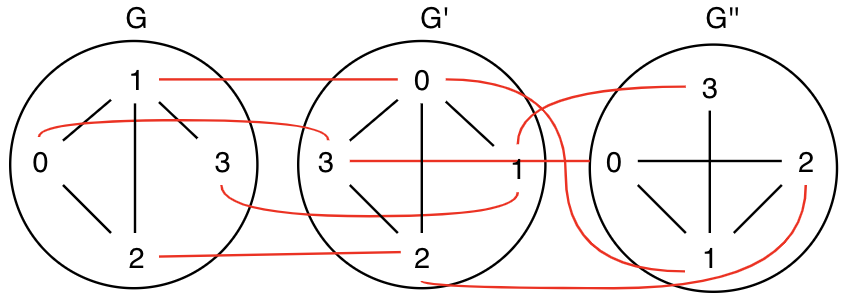
\includegraphics[width=6cm]{images/esempio-isomorfismo.png}
        \vspace{-8pt}
        \caption{}
    \end{subfigure}
    \hspace{3cm}
    \begin{subfigure}{.3\textwidth}
        \centering
        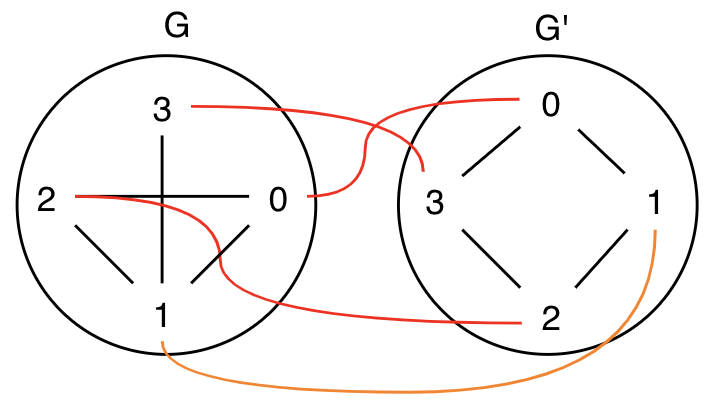
\includegraphics[width=4.5cm]{images/es-non-isomorfmismo.png}
        \vspace{-5pt}
        \caption{}
    \end{subfigure}
    \vspace{-5pt}
    \caption{(a) Esempio Isomorfismo, (b) Esempio non isomorfismo}
\end{figure}

\subsection{Grafi notevoli}
Esistono una serie di grafi, detti grafi notevoli, che per la loro struttura particolare hanno preso dei nomi specifici, essi possono essere anche ritrovati di frequente in differenti casistiche in cui si utilizzano grafi.
\begin{figure}[h!]
    \vspace{-10pt}
    \begin{subfigure}{.3\textwidth}
        \centering
        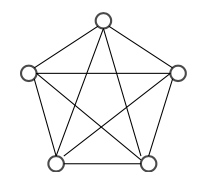
\includegraphics[width=3cm]{images/clinque.png}
        \vspace{-5pt}
        \caption{Clinque}
    \end{subfigure}
    \hfill
    \begin{subfigure}{.3\textwidth}
        \centering
        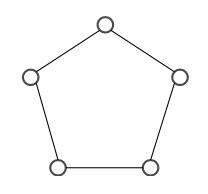
\includegraphics[width=2.5cm]{images/ciclo.png}
        \vspace{-5pt}
        \caption{Ciclo}
    \end{subfigure}
    \hfill
    \begin{subfigure}{.3\textwidth}
        \centering
        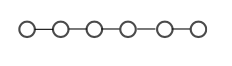
\includegraphics[width=2.5cm]{images/lineare.png}
        \vspace{-5pt}
        \caption{Lineare}
    \end{subfigure}
    \hfill
    \begin{subfigure}{.3\textwidth}
        \centering
        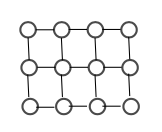
\includegraphics[width=2.5cm]{images/griglia.png}
        \vspace{-5pt}
        \caption{Griglia}
    \end{subfigure}
    \hfill
    \begin{subfigure}{.3\textwidth}
        \centering
        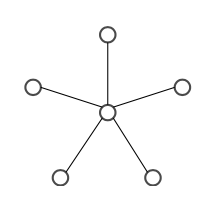
\includegraphics[width=2.5cm]{images/stella.png}
        \vspace{-5pt}
        \caption{Stella}
    \end{subfigure}
    \hfill
    \begin{subfigure}{.3\textwidth}
        \centering
        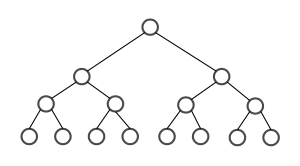
\includegraphics[width=2.5cm]{images/albero-completo.png}
        \vspace{-5pt}
        \caption{Albero completo}
    \end{subfigure}
    \vspace{5pt}
    \caption{Serie di grafi notevoli}
\end{figure}